% Created by tikzDevice version 0.12 on 2019-04-08 10:07:46
% !TEX encoding = UTF-8 Unicode
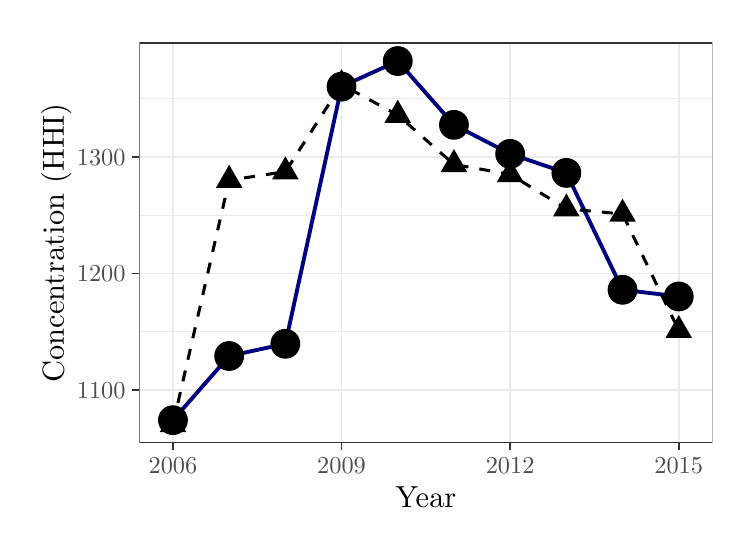
\begin{tikzpicture}[x=1pt,y=1pt]
\definecolor{fillColor}{RGB}{255,255,255}
\path[use as bounding box,fill=fillColor,fill opacity=0.00] (0,0) rectangle (252.94,180.67);
\begin{scope}
\path[clip] (  0.00,  0.00) rectangle (252.94,180.67);
\definecolor{drawColor}{RGB}{255,255,255}
\definecolor{fillColor}{RGB}{255,255,255}

\path[draw=drawColor,line width= 0.6pt,line join=round,line cap=round,fill=fillColor] (  0.00, -0.00) rectangle (252.94,180.67);
\end{scope}
\begin{scope}
\path[clip] ( 40.32, 30.72) rectangle (247.44,175.17);
\definecolor{fillColor}{RGB}{255,255,255}

\path[fill=fillColor] ( 40.32, 30.72) rectangle (247.45,175.17);
\definecolor{drawColor}{gray}{0.92}

\path[draw=drawColor,line width= 0.3pt,line join=round] ( 40.32, 70.77) --
	(247.44, 70.77);

\path[draw=drawColor,line width= 0.3pt,line join=round] ( 40.32,112.87) --
	(247.44,112.87);

\path[draw=drawColor,line width= 0.3pt,line join=round] ( 40.32,154.97) --
	(247.44,154.97);

\path[draw=drawColor,line width= 0.6pt,line join=round] ( 40.32, 49.72) --
	(247.44, 49.72);

\path[draw=drawColor,line width= 0.6pt,line join=round] ( 40.32, 91.82) --
	(247.44, 91.82);

\path[draw=drawColor,line width= 0.6pt,line join=round] ( 40.32,133.92) --
	(247.44,133.92);

\path[draw=drawColor,line width= 0.6pt,line join=round] ( 52.50, 30.72) --
	( 52.50,175.17);

\path[draw=drawColor,line width= 0.6pt,line join=round] (113.42, 30.72) --
	(113.42,175.17);

\path[draw=drawColor,line width= 0.6pt,line join=round] (174.34, 30.72) --
	(174.34,175.17);

\path[draw=drawColor,line width= 0.6pt,line join=round] (235.26, 30.72) --
	(235.26,175.17);
\definecolor{drawColor}{RGB}{0,0,128}

\path[draw=drawColor,line width= 1.4pt,line join=round] ( 52.50, 38.85) --
	( 72.81, 62.03) --
	( 93.11, 66.44) --
	(113.42,159.36) --
	(133.73,168.61) --
	(154.03,145.55) --
	(174.34,135.07) --
	(194.65,128.19) --
	(214.95, 85.95) --
	(235.26, 83.54);
\definecolor{drawColor}{RGB}{0,0,0}
\definecolor{fillColor}{RGB}{0,0,0}

\path[draw=drawColor,line width= 0.4pt,line join=round,line cap=round,fill=fillColor] ( 52.50, 38.85) circle (  5.18);

\path[draw=drawColor,line width= 0.4pt,line join=round,line cap=round,fill=fillColor] ( 72.81, 62.03) circle (  5.18);

\path[draw=drawColor,line width= 0.4pt,line join=round,line cap=round,fill=fillColor] ( 93.11, 66.44) circle (  5.18);

\path[draw=drawColor,line width= 0.4pt,line join=round,line cap=round,fill=fillColor] (113.42,159.36) circle (  5.18);

\path[draw=drawColor,line width= 0.4pt,line join=round,line cap=round,fill=fillColor] (133.73,168.61) circle (  5.18);

\path[draw=drawColor,line width= 0.4pt,line join=round,line cap=round,fill=fillColor] (154.03,145.55) circle (  5.18);

\path[draw=drawColor,line width= 0.4pt,line join=round,line cap=round,fill=fillColor] (174.34,135.07) circle (  5.18);

\path[draw=drawColor,line width= 0.4pt,line join=round,line cap=round,fill=fillColor] (194.65,128.19) circle (  5.18);

\path[draw=drawColor,line width= 0.4pt,line join=round,line cap=round,fill=fillColor] (214.95, 85.95) circle (  5.18);

\path[draw=drawColor,line width= 0.4pt,line join=round,line cap=round,fill=fillColor] (235.26, 83.54) circle (  5.18);

\path[draw=drawColor,line width= 1.1pt,dash pattern=on 4pt off 4pt ,line join=round] ( 52.50, 37.29) --
	( 72.81,125.55) --
	( 93.11,128.63) --
	(113.42,160.11) --
	(133.73,149.07) --
	(154.03,131.25) --
	(174.34,127.66) --
	(194.65,115.23) --
	(214.95,113.33) --
	(235.26, 71.32);

\path[fill=fillColor] ( 52.50, 42.84) --
	( 57.31, 34.52) --
	( 47.69, 34.52) --
	cycle;

\path[fill=fillColor] ( 72.81,131.10) --
	( 77.61,122.78) --
	( 68.00,122.78) --
	cycle;

\path[fill=fillColor] ( 93.11,134.18) --
	( 97.92,125.86) --
	( 88.31,125.86) --
	cycle;

\path[fill=fillColor] (113.42,165.66) --
	(118.23,157.33) --
	(108.61,157.33) --
	cycle;

\path[fill=fillColor] (133.73,154.62) --
	(138.53,146.29) --
	(128.92,146.29) --
	cycle;

\path[fill=fillColor] (154.03,136.80) --
	(158.84,128.48) --
	(149.23,128.48) --
	cycle;

\path[fill=fillColor] (174.34,133.21) --
	(179.15,124.88) --
	(169.53,124.88) --
	cycle;

\path[fill=fillColor] (194.65,120.78) --
	(199.45,112.46) --
	(189.84,112.46) --
	cycle;

\path[fill=fillColor] (214.95,118.88) --
	(219.76,110.56) --
	(210.15,110.56) --
	cycle;

\path[fill=fillColor] (235.26, 76.87) --
	(240.07, 68.54) --
	(230.45, 68.54) --
	cycle;
\definecolor{drawColor}{gray}{0.20}

\path[draw=drawColor,line width= 0.6pt,line join=round,line cap=round] ( 40.32, 30.72) rectangle (247.45,175.17);
\end{scope}
\begin{scope}
\path[clip] (  0.00,  0.00) rectangle (252.94,180.67);
\definecolor{drawColor}{gray}{0.30}

\node[text=drawColor,anchor=base east,inner sep=0pt, outer sep=0pt, scale=  0.88] at ( 35.37, 46.69) {1100};

\node[text=drawColor,anchor=base east,inner sep=0pt, outer sep=0pt, scale=  0.88] at ( 35.37, 88.79) {1200};

\node[text=drawColor,anchor=base east,inner sep=0pt, outer sep=0pt, scale=  0.88] at ( 35.37,130.89) {1300};
\end{scope}
\begin{scope}
\path[clip] (  0.00,  0.00) rectangle (252.94,180.67);
\definecolor{drawColor}{gray}{0.20}

\path[draw=drawColor,line width= 0.6pt,line join=round] ( 37.57, 49.72) --
	( 40.32, 49.72);

\path[draw=drawColor,line width= 0.6pt,line join=round] ( 37.57, 91.82) --
	( 40.32, 91.82);

\path[draw=drawColor,line width= 0.6pt,line join=round] ( 37.57,133.92) --
	( 40.32,133.92);
\end{scope}
\begin{scope}
\path[clip] (  0.00,  0.00) rectangle (252.94,180.67);
\definecolor{drawColor}{gray}{0.20}

\path[draw=drawColor,line width= 0.6pt,line join=round] ( 52.50, 27.97) --
	( 52.50, 30.72);

\path[draw=drawColor,line width= 0.6pt,line join=round] (113.42, 27.97) --
	(113.42, 30.72);

\path[draw=drawColor,line width= 0.6pt,line join=round] (174.34, 27.97) --
	(174.34, 30.72);

\path[draw=drawColor,line width= 0.6pt,line join=round] (235.26, 27.97) --
	(235.26, 30.72);
\end{scope}
\begin{scope}
\path[clip] (  0.00,  0.00) rectangle (252.94,180.67);
\definecolor{drawColor}{gray}{0.30}

\node[text=drawColor,anchor=base,inner sep=0pt, outer sep=0pt, scale=  0.88] at ( 52.50, 19.71) {2006};

\node[text=drawColor,anchor=base,inner sep=0pt, outer sep=0pt, scale=  0.88] at (113.42, 19.71) {2009};

\node[text=drawColor,anchor=base,inner sep=0pt, outer sep=0pt, scale=  0.88] at (174.34, 19.71) {2012};

\node[text=drawColor,anchor=base,inner sep=0pt, outer sep=0pt, scale=  0.88] at (235.26, 19.71) {2015};
\end{scope}
\begin{scope}
\path[clip] (  0.00,  0.00) rectangle (252.94,180.67);
\definecolor{drawColor}{RGB}{0,0,0}

\node[text=drawColor,anchor=base,inner sep=0pt, outer sep=0pt, scale=  1.10] at (143.88,  7.44) {Year};
\end{scope}
\begin{scope}
\path[clip] (  0.00,  0.00) rectangle (252.94,180.67);
\definecolor{drawColor}{RGB}{0,0,0}

\node[text=drawColor,rotate= 90.00,anchor=base,inner sep=0pt, outer sep=0pt, scale=  1.10] at ( 13.08,102.95) {Concentration (HHI)};
\end{scope}
\end{tikzpicture}
